\subsection{Implementation}
% 
In the the prototype, we use the architecture described in Figure \ref{fig:arch-ver2-tech} as the basics for our system design. In this section //TO BE WRITTEN: SECTION OVERVIEW

The idea of the project -- to exchange cryptocurrencies -- is too broad to be implemented without further refinements. To be able to implement the prototype, we need to break this idea down to a list of desired functions or functional requirements. 

In a usual software development process, functional requirements would come from the users of the system, product owner and other stakeholders. In this project, we list the requirements for the prototype, so that the idea can be demonstrated clearly. Requirements necessary for demonstrating the idea were prioritised, the others were not worked upon. We ranked the requirements by their importance and then sorted them in a MoSCoW table. We used this table to prioritise the areas for implementation. In a market-ready product, many requirements would most likely be different.

In the previous examples, we have always considered that the two trading parties -- Alice and Bob agreed on the terms of the transaction beforehand using a separate channel. For this prototype, we have decided to include a communication channel, to enable users interact and agree on the transaction terms within the prototype. While this functionality is certainly not novel, nor it is the focus of this project, it complements the prototype and showcases, how it could be used in real-world.

\subsubsection{System parts}
The prototype is implemented as an Android application. It communicates with Ethereum blockchain via Ethereum node, to deploy a custom smart contract, which operates logic described in figure \ref{fig:simple-logic} on page \pageref{fig:simple-logic} and with a back-end that facilitates the communication channel. To operate its logic, the smart contract communicates with an oracle. The oracle queries a blockchain explorer provider to learn about the status of a transaction and sends the updates back to the smart contract. User triggers the events in the Android application and validates events on the blockchain. The validation should be done with use of other systems than the Android application itself. Figure \ref{fig:system-overview} depicts the system parts and their relations. 
% 
\begin{figure}[p]
    \centering
    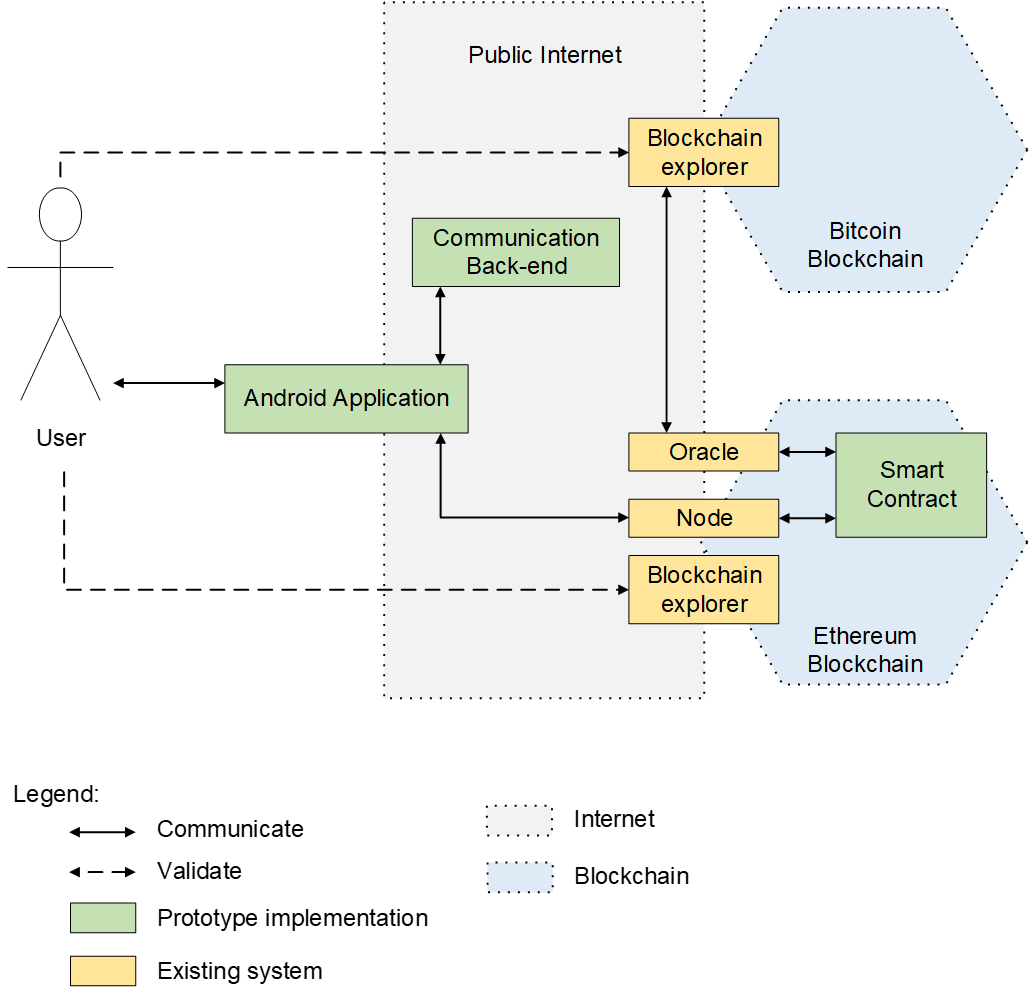
\includegraphics[width=\textwidth]{system-overview}
    \caption[itemize]{
    Overview of the system parts:
    \begin{itemize}[nolistsep, noitemsep]
        \item \textit{User} communicates directly with the Android application and verifies data on the blockchain.
        \item \textit{Android application} fetches data about existing offers from the communication back-end and sends new smart contracts to the Ethereum node.
        \item \textit{Node} communicates with other nodes in the Ethereum network, maintains the status of the blockchain and deploys new smart contracts to the network.
        \item \textit{Smart contract} contacts oracle after deployment and holds the funds until the oracle has cleared the transaction as approved.
        \item The \textit{oracle} queries the Bitcoin block explorer to learn about the status of the transaction and communicates the result back to the smart contract.
    \end{itemize}
    }
    \label{fig:system-overview}
\end{figure}

//Further details about implementation of every system in the figure will follow here.
% 
\paragraph{Android Application} 
Using Android XX and using mainly fragments for interface and wrappers for other stuff and QR code and Firebase etc...
Using Java (as opposed to Kotlin) etc.
% 
\paragraph{Node}
Running an Infura node, because it's...
% 
\paragraph{Smart Contract}
Properties of the smart contract, written in Solidity, emitting events...
% 
\paragraph{Oracle}
Using Oraclize for this service... why? Why not?
% 
\paragraph{Blockchain explorer}
Using blockchain.info... why? Why not?


\subsubsection{Prototype requirements}

//HERE: MoSCoW with requirements (probably?)

\subsubsection{Flows/usage}
% 
In this section we will showcase how the app is used - what data is entered when, what screens are presented -- not sure how important is to have this.


